\section{Backup}

% CUE A1 | Q&A 백업: 성과 평가지표의 계량적 정의
\begin{frame}{[백업 A1] 성과 평가지표의 계량적 정의 및 샤프 산출 기준}
\textbf{핵심 계량 지표의 수학적 정의 (논문 식 33a $\sim$ 33c)}:
\begin{equation*}
  \text{CAGR} = \left(\frac{V_T}{V_0}\right)^{\frac{252}{T}} - 1, \quad
  \sigma_{\text{ann}} = \sqrt{252} \times \sqrt{\frac{1}{T-1}\sum_{t=1}^T (r_t - \bar{r})^2}
\end{equation*}
\begin{equation*}
  \text{Sharpe Ratio} = \frac{\mu_{\text{ann}} - r_f}{\sigma_{\text{ann}}}, \quad
  \text{Sortino Ratio} = \frac{\mu_{\text{ann}} - r_f}{\sqrt{252 \cdot \text{LPM}_2}}, \quad
  \text{Calmar Ratio} = \frac{\text{CAGR}}{|\text{MDD}|}
\end{equation*}

\vspace{1mm}
\begin{block}{샤프 지수 분자 기준에 관한 엄밀한 설명}
  \small
  \begin{itemize}
    \item \textbf{이론적 정의}: 산술평균 분자 적용 시 $\text{SR} = (15.11\% - 2.0\%) / 7.63\% = \mathbf{1.72}$
    \item \textbf{표 2 보고 기준}: 복리 기하수익률(CAGR)을 분자로 적용하여 더욱 보수적으로 산출:
    $\text{SR} = (14.82\% - 2.0\%) / 7.63\% = \mathbf{1.68}$
    \item 투자자의 실제 실현 복리 부(Terminal Wealth) 관점에서 보수적 지표를 보고함.
  \end{itemize}
\end{block}
\end{frame}

% CUE A2 | Q&A 백업: Ledoit-Wolf 축소 및 Higham PSD 사영
\begin{frame}{[백업 A2] 공분산 행렬 정규화: Ledoit-Wolf 축소 및 Higham 사영}
\textbf{1. 르두아-울프 (Ledoit-Wolf, 2004) 축소 추정량}:
\begin{equation*}
  \hat{\boldsymbol{\Sigma}}_{\text{LW}} = (1 - \hat{\delta}) \mathbf{S} + \hat{\delta} \mathbf{F}
\end{equation*}
여기서 $\mathbf{S}$는 표본 공분산 행렬, $\mathbf{F}$는 1-파라미터 등분산 타겟(Equicorrelation Target), $\hat{\delta} \in [0, 1]$는 점근적 최적 축소 강도(Optimal Shrinkage Intensity)임.

\vspace{3mm}
\textbf{2. 하이엄 (Higham, 2002) 최근접 상관행렬 교대 투영법}:
\begin{equation*}
  \hat{\mathbf{C}}_{k+1} = \mathcal{P}_S \left( \mathcal{P}_U (\hat{\mathbf{C}}_k) \right)
\end{equation*}
\begin{itemize}
  \small
  \item $\mathcal{P}_U$: 대각 성분을 1로 투영하는 단위 대각화 사영.
  \item $\mathcal{P}_S$: 음(-)의 고유값을 잘라내고 양준정부호 콘(Positive Semidefinite Cone) 위로 투영하는 스펙트럴 사영.
  \item 최종 복원 공분산 행렬: $\hat{\boldsymbol{\Sigma}}_t = \mathbf{D}^{\frac{1}{2}} \hat{\mathbf{C}}_\infty \mathbf{D}^{\frac{1}{2}} \succ 0$ (볼록 최적화 실행 타당성 보장).
\end{itemize}
\end{frame}

% CUE A3 | Q&A 백업: 거래비용 수준별 민감도 종합 대조표
\begin{frame}{[백업 A3] 거래비용 수준별 성과 민감도: 제출본 vs 실데이터}
\small
\begin{table}[H]
\centering
\begin{tabular}{lcccc}
\toprule
\textbf{편도 거래비용} & \textbf{제출본 시뮬레이션} & \textbf{제출본 샤프} & \textbf{실데이터 (Primary)} & \textbf{실데이터 샤프} \\
\midrule
\textbf{0 bp (수수료 無)} & 14.82\% & 1.68 & \textbf{15.11\%} & \textbf{1.16} \\
\textbf{5 bp (대형 기금)} & 14.73\% & 1.67 & — & — \\
\textbf{10 bp (기본 비용)} & 14.63\% & 1.65 & \textbf{11.91\%} & \textbf{0.90} \\
\textbf{15 bp (보수적)} & 14.54\% & 1.64 & — & — \\
\textbf{20 bp (고비용 스트레스)} & 14.44\% & 1.63 & \textbf{8.81\%} & \textbf{0.64} \\
\bottomrule
\end{tabular}
\end{table}

\begin{block}{시사점 분석}
  \small
  \begin{itemize}
    \item \textbf{수수료가 없을 때(0bp)}: 실데이터에서도 제안 모델은 연평균 복리수익률 \textbf{15.11\%}, 샤프 \textbf{1.16}으로 60/40(10.37\%) 대비 강력한 알파를 창출함.
    \item \textbf{비용 증가 시}: 주간 재최적화에 따른 높은 연간 회전율(2,804\%)로 인해 거래비용 마찰이 가속되어 초과성과가 감소함 $\rightarrow$ 차기 연구에서 \textbf{회전율 제약 목적함수} 도입의 정당성 확보 (탐색 분석: 백업 A8).
  \end{itemize}
\end{block}
\end{frame}

% CUE A4 | Q&A 백업: 실데이터 6대 전략 전체 성과표
\begin{frame}{[백업 A4] 실데이터 사전등록 재현: 6대 전략 전체 성과표}
\scriptsize
\textbf{Primary 외표본 평가 기간 (2017.01 $\sim$ 2026.08, 거래비용 10bp)}:
\begin{table}[H]
\centering
\begin{tabular}{lcccccccc}
\toprule
\textbf{전략} & \textbf{CAGR} & \textbf{$\sigma$} & \textbf{Sharpe} & \textbf{MDD} & \textbf{회전율} & \textbf{실측 항력} & \textbf{$\frac{1}{2}\sigma^2$} & \textbf{JB 검정} \\
\midrule
전통적 60/40 & 10.37\% & 11.61\% & 0.77 & -19.18\% & 20.7\% & 0.68\% & 0.67\% & 2,868일 기각 \\
동일가중 (1/N) & 12.93\% & 11.63\% & 0.98 & -17.51\% & 39.2\% & 0.68\% & 0.68\% & 정규성 기각 \\
마코위츠 MVO & 12.89\% & 12.52\% & 0.91 & -15.17\% & 835.0\% & 0.79\% & 0.78\% & 정규성 기각 \\
이토-켈리 (과거 모멘트) & 12.70\% & 12.91\% & 0.88 & -19.24\% & 660.2\% & 0.84\% & 0.83\% & 정규성 기각 \\
이토-켈리 + Chronos & \textbf{13.97\%} & 12.55\% & \textbf{0.99} & -20.06\% & 2,656\% & 0.79\% & 0.79\% & 정규성 기각 \\
\textbf{제안 모델 (통합)} & 11.91\% & \textbf{11.56\%} & 0.90 & -19.67\% & 2,804\% & \textbf{0.67\%} & \textbf{0.67\%} & 정규성 기각 \\
\bottomrule
\end{tabular}
\end{table}

\begin{itemize}
  \tiny
  \item \textbf{소거 실험(Ablation)}: TSFM(Chronos) 결합 시 샤프 지수가 0.88 $\rightarrow$ 0.99로 상승하여 파운데이션 모델의 1차·2차 모멘트 예측 기여 입증.
  \item \textbf{항력 일치성}: 모든 전략에서 실측 변동성 항력($\mu - g$)과 이론치($\frac{1}{2}\sigma^2$)가 0.01\%p 이내로 완벽 부합.
\end{itemize}
\end{frame}

% CUE A5 | Q&A 백업: 미래참조편향 차단 설계
\begin{frame}{[백업 A5] 미래참조편향(Look-ahead Bias) 차단 및 테스트}
\begin{columns}[T]
  \begin{column}{0.48\textwidth}
    \textbf{1. 시점별 정보집합 ($\mathcal{F}_t$) 가측성}
    \begin{itemize}
      \setlength{\itemsep}{3pt}
      \small
      \item 미국/환율(FX) 자산은 KRX 개장일 직전 거래일 종가만을 결합.
      \item RevIN 정규화의 평균·표준편차는 윈도우 $[t-L, t]$ 데이터로만 산출.
      \item $t$ 시점 종가로 결정된 목표 가중치는 $t+1$ 시점부터 수익률을 수취함.
    \end{itemize}
  \end{column}
  
  \begin{column}{0.48\textwidth}
    \textbf{2. 오토인코더 사전학습 동결}
    \begin{itemize}
      \setlength{\itemsep}{3pt}
      \small
      \item 2015~2016년 웜업 데이터만으로 정상 매니폴드를 사전학습한 후 가중치를 영구 동결.
      \item 2017년 이후 외표본 구간에서는 미래 위기 데이터를 참조하지 않음.
    \end{itemize}
  \end{column}
\end{columns}

\vspace{3mm}
\begin{exampleblock}{단위 테스트 검증 (\texttt{tests/test\_pipeline.py})}
  \small 미래 시점의 자산 가격을 인위적으로 변조(Shuffling)한 후 $t$ 시점의 최적 가중치를 재산출하였을 때, 가중치 벡터가 1e-12 오차 이내로 완전히 동일함을 확인하는 불변성 단위 테스트 통과.
\end{exampleblock}
\end{frame}

% CUE A6 | Q&A 백업: 주최측 합의 서지 정정 내역
\begin{frame}{[백업 A6] 주최측 합의 서지 정보 정정 내역 (10/5 학생회 메일)}
\small
\begin{table}[H]
\centering
\begin{tabular}{lp{5.5cm}p{5.5cm}}
\toprule
\textbf{항목} & \textbf{기제출본 표기} & \textbf{공식 정정 서지 (정합성 완결)} \\
\midrule
\textbf{Hallerbach (2014)} & 저널 정보 및 DOI 표기 누락 & \textit{Journal of Asset Management}, Vol. 15, No. 5, pp. 281--287. 공식 DOI 확인. \\
\midrule
\textbf{Das et al. (2024)} & Google TimesFM 인용 시 프로시딩 수록 페이지 누락 & \textit{ICML 2024 (PMLR)}, Vol. 235, pp. 10148--10167. 권호 및 페이지 완결. \\
\midrule
\textbf{Itô's Lemma} & 관용적 교과서 인용 & \textbf{Itô, K. (1951)}, ``On stochastic differential equations'', \textit{Nagoya Math. J.}, Vol. 3, pp. 55--65 원전 명시. \\
\bottomrule
\end{tabular}
\end{table}

\begin{block}{학술제 주최측과의 사전 협의 완료}
  \small 서강대 학생회 제36대 [Loop] 학술국장과의 공식 협의(10/5)에 따라, 심사위원 사전 배부본과의 형평성을 유지하면서 본선 발표자료에서 위 서지 정정 사항을 정식 반영하여 보고함.
\end{block}
\end{frame}

% CUE A7 | Q&A 백업: 주요 참고문헌
\begin{frame}[allowframebreaks]{[백업 A7] 주요 참고문헌 (References)}
\scriptsize
\nocite{*}
\bibliography{Mybib}
\end{frame}

% CUE A8 | Q&A 백업 (p.27): L1 회전율 페널티 탐색 분석 — 사전등록 외
% Figure: alphaquant-tsfm-voldrag-empirical/scripts/generate_backup_slide27_chart.py
\begin{frame}{[백업 A8] L1 회전율 페널티: 탐색 분석 (사전등록 외)}
\centering
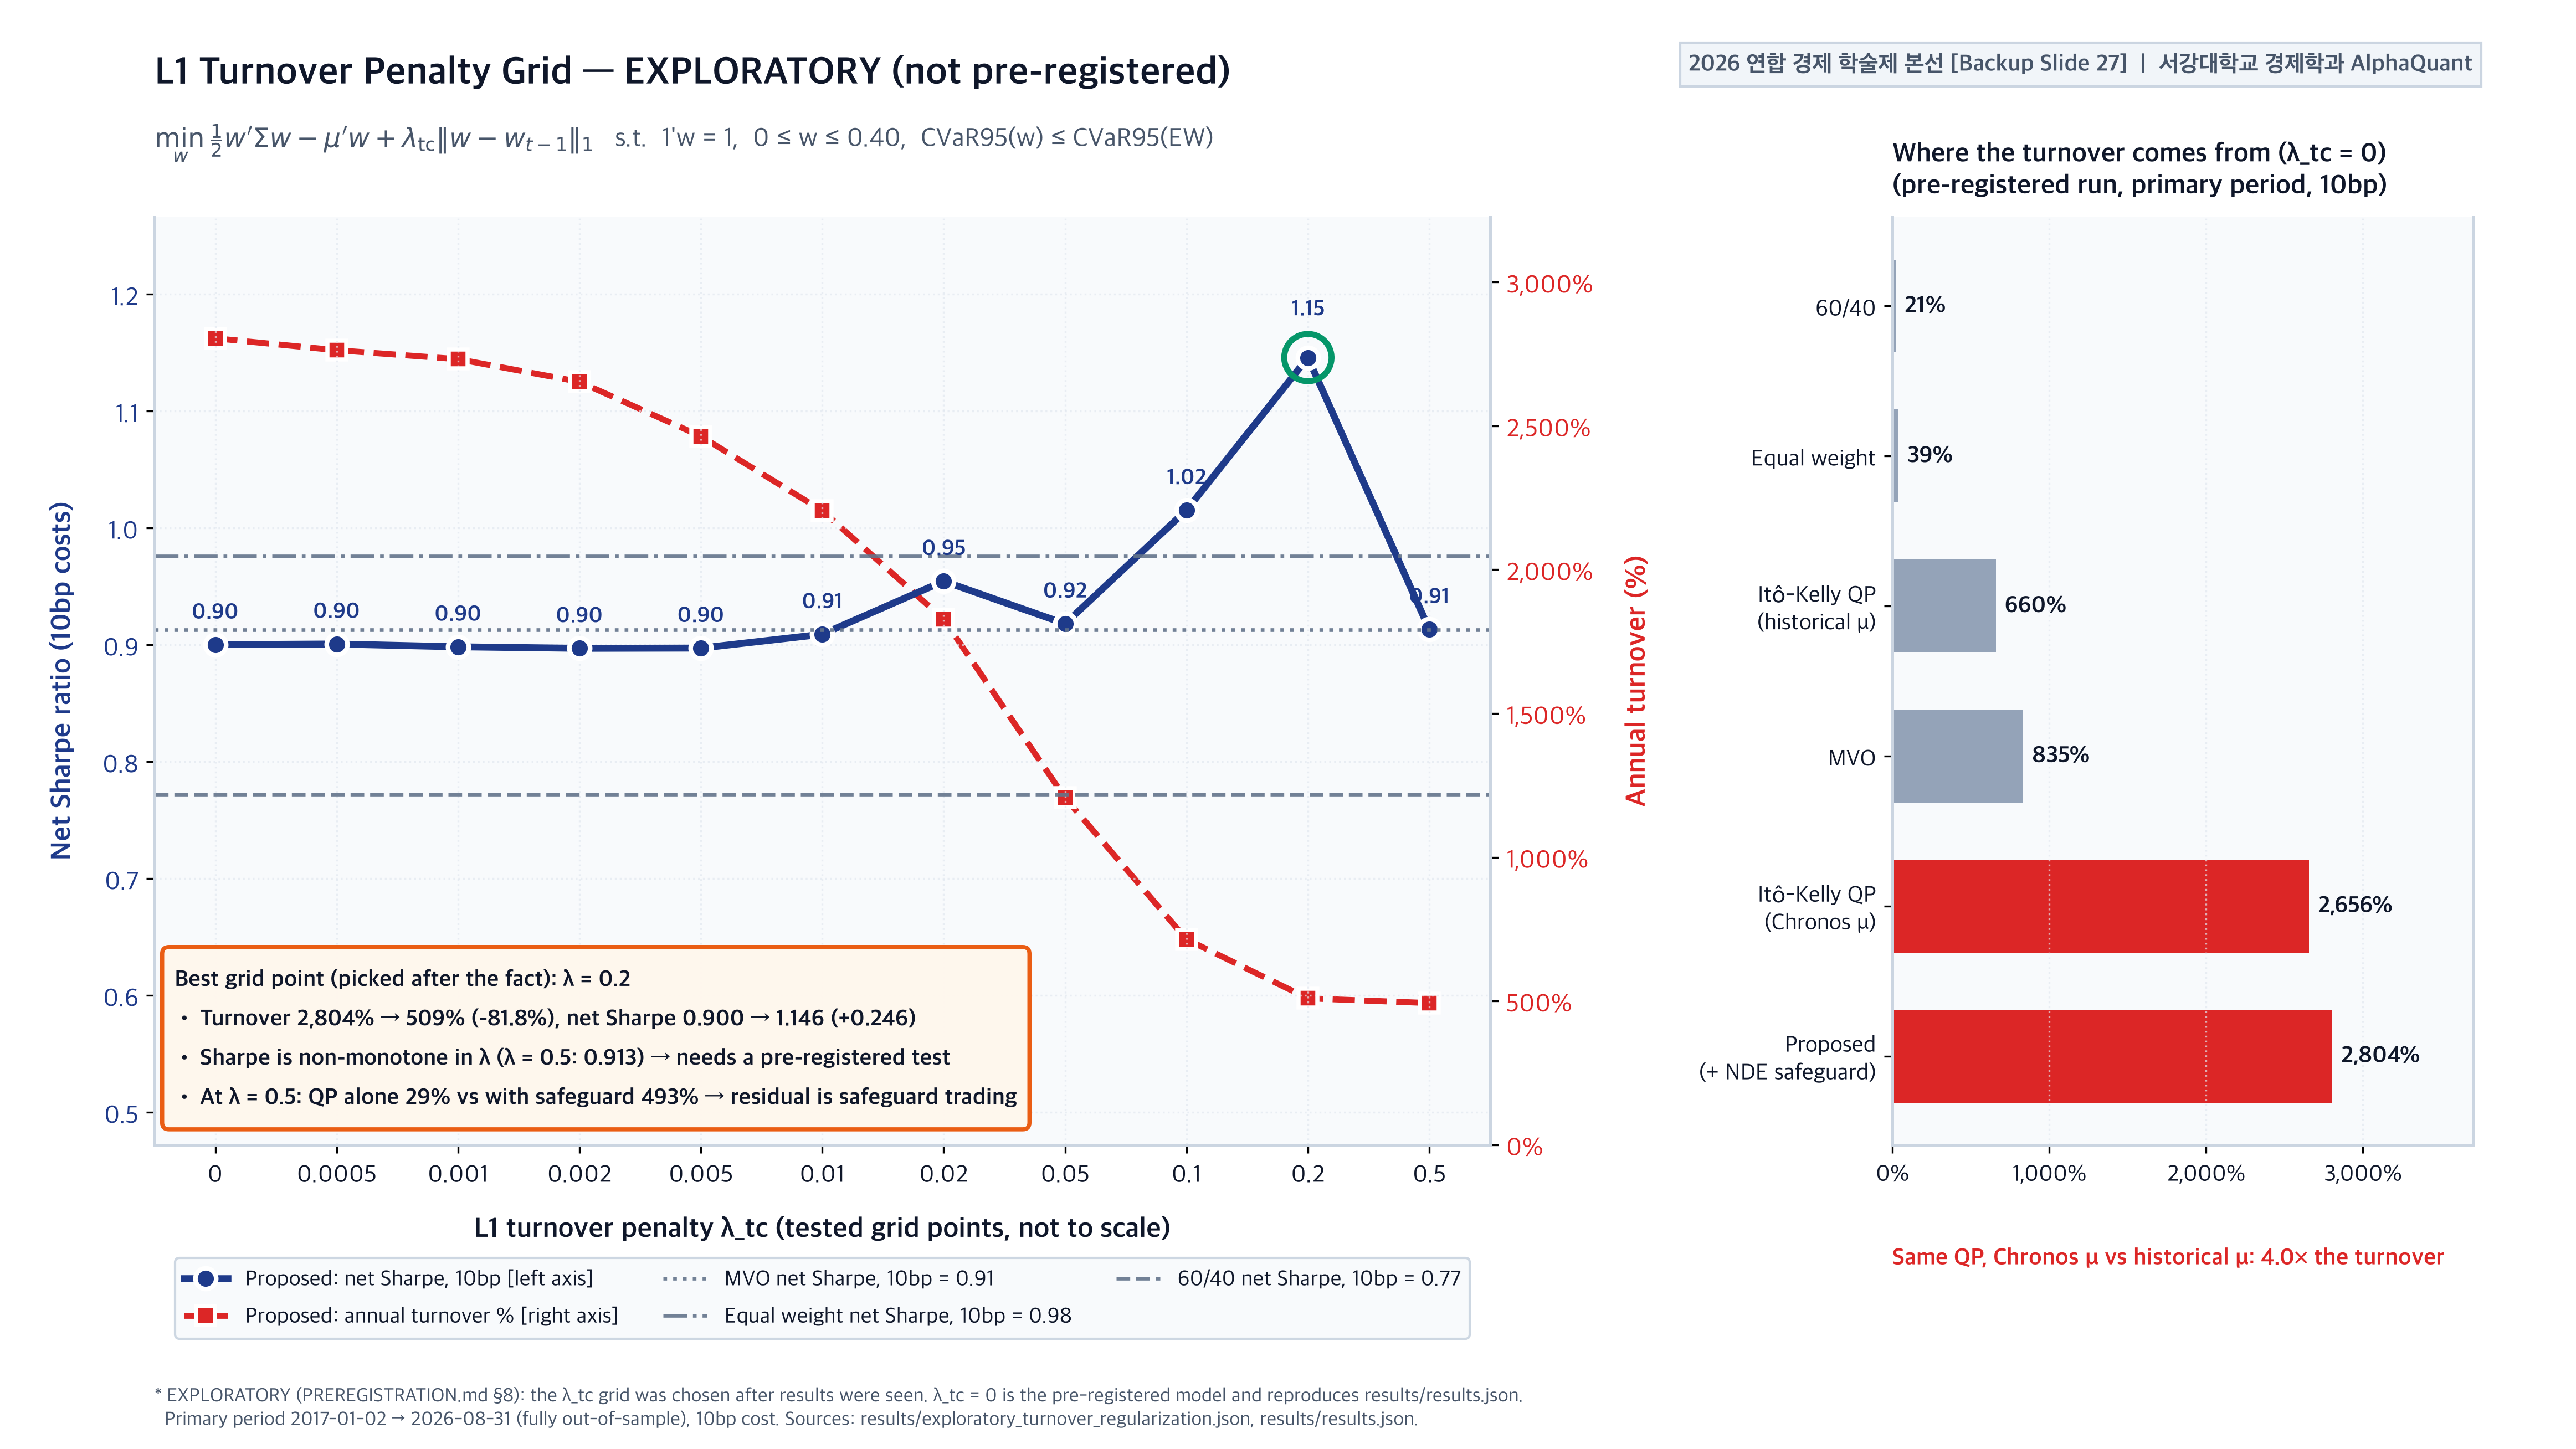
\includegraphics[width=\linewidth,height=0.86\textheight,keepaspectratio]{MyFigure/backup_slide27_turnover_frontier.png}
\end{frame}
